\section{Results}
\label{Results}
%\section{Data Analysis}
%\label{Data Analysis}

\subsection{Flight Data}
%Notes on how to take the results...
%What is being presented: Five plots total, the flight profile for each year, and cumulative dose for each flight.

\begin{figure}[H]
\centering
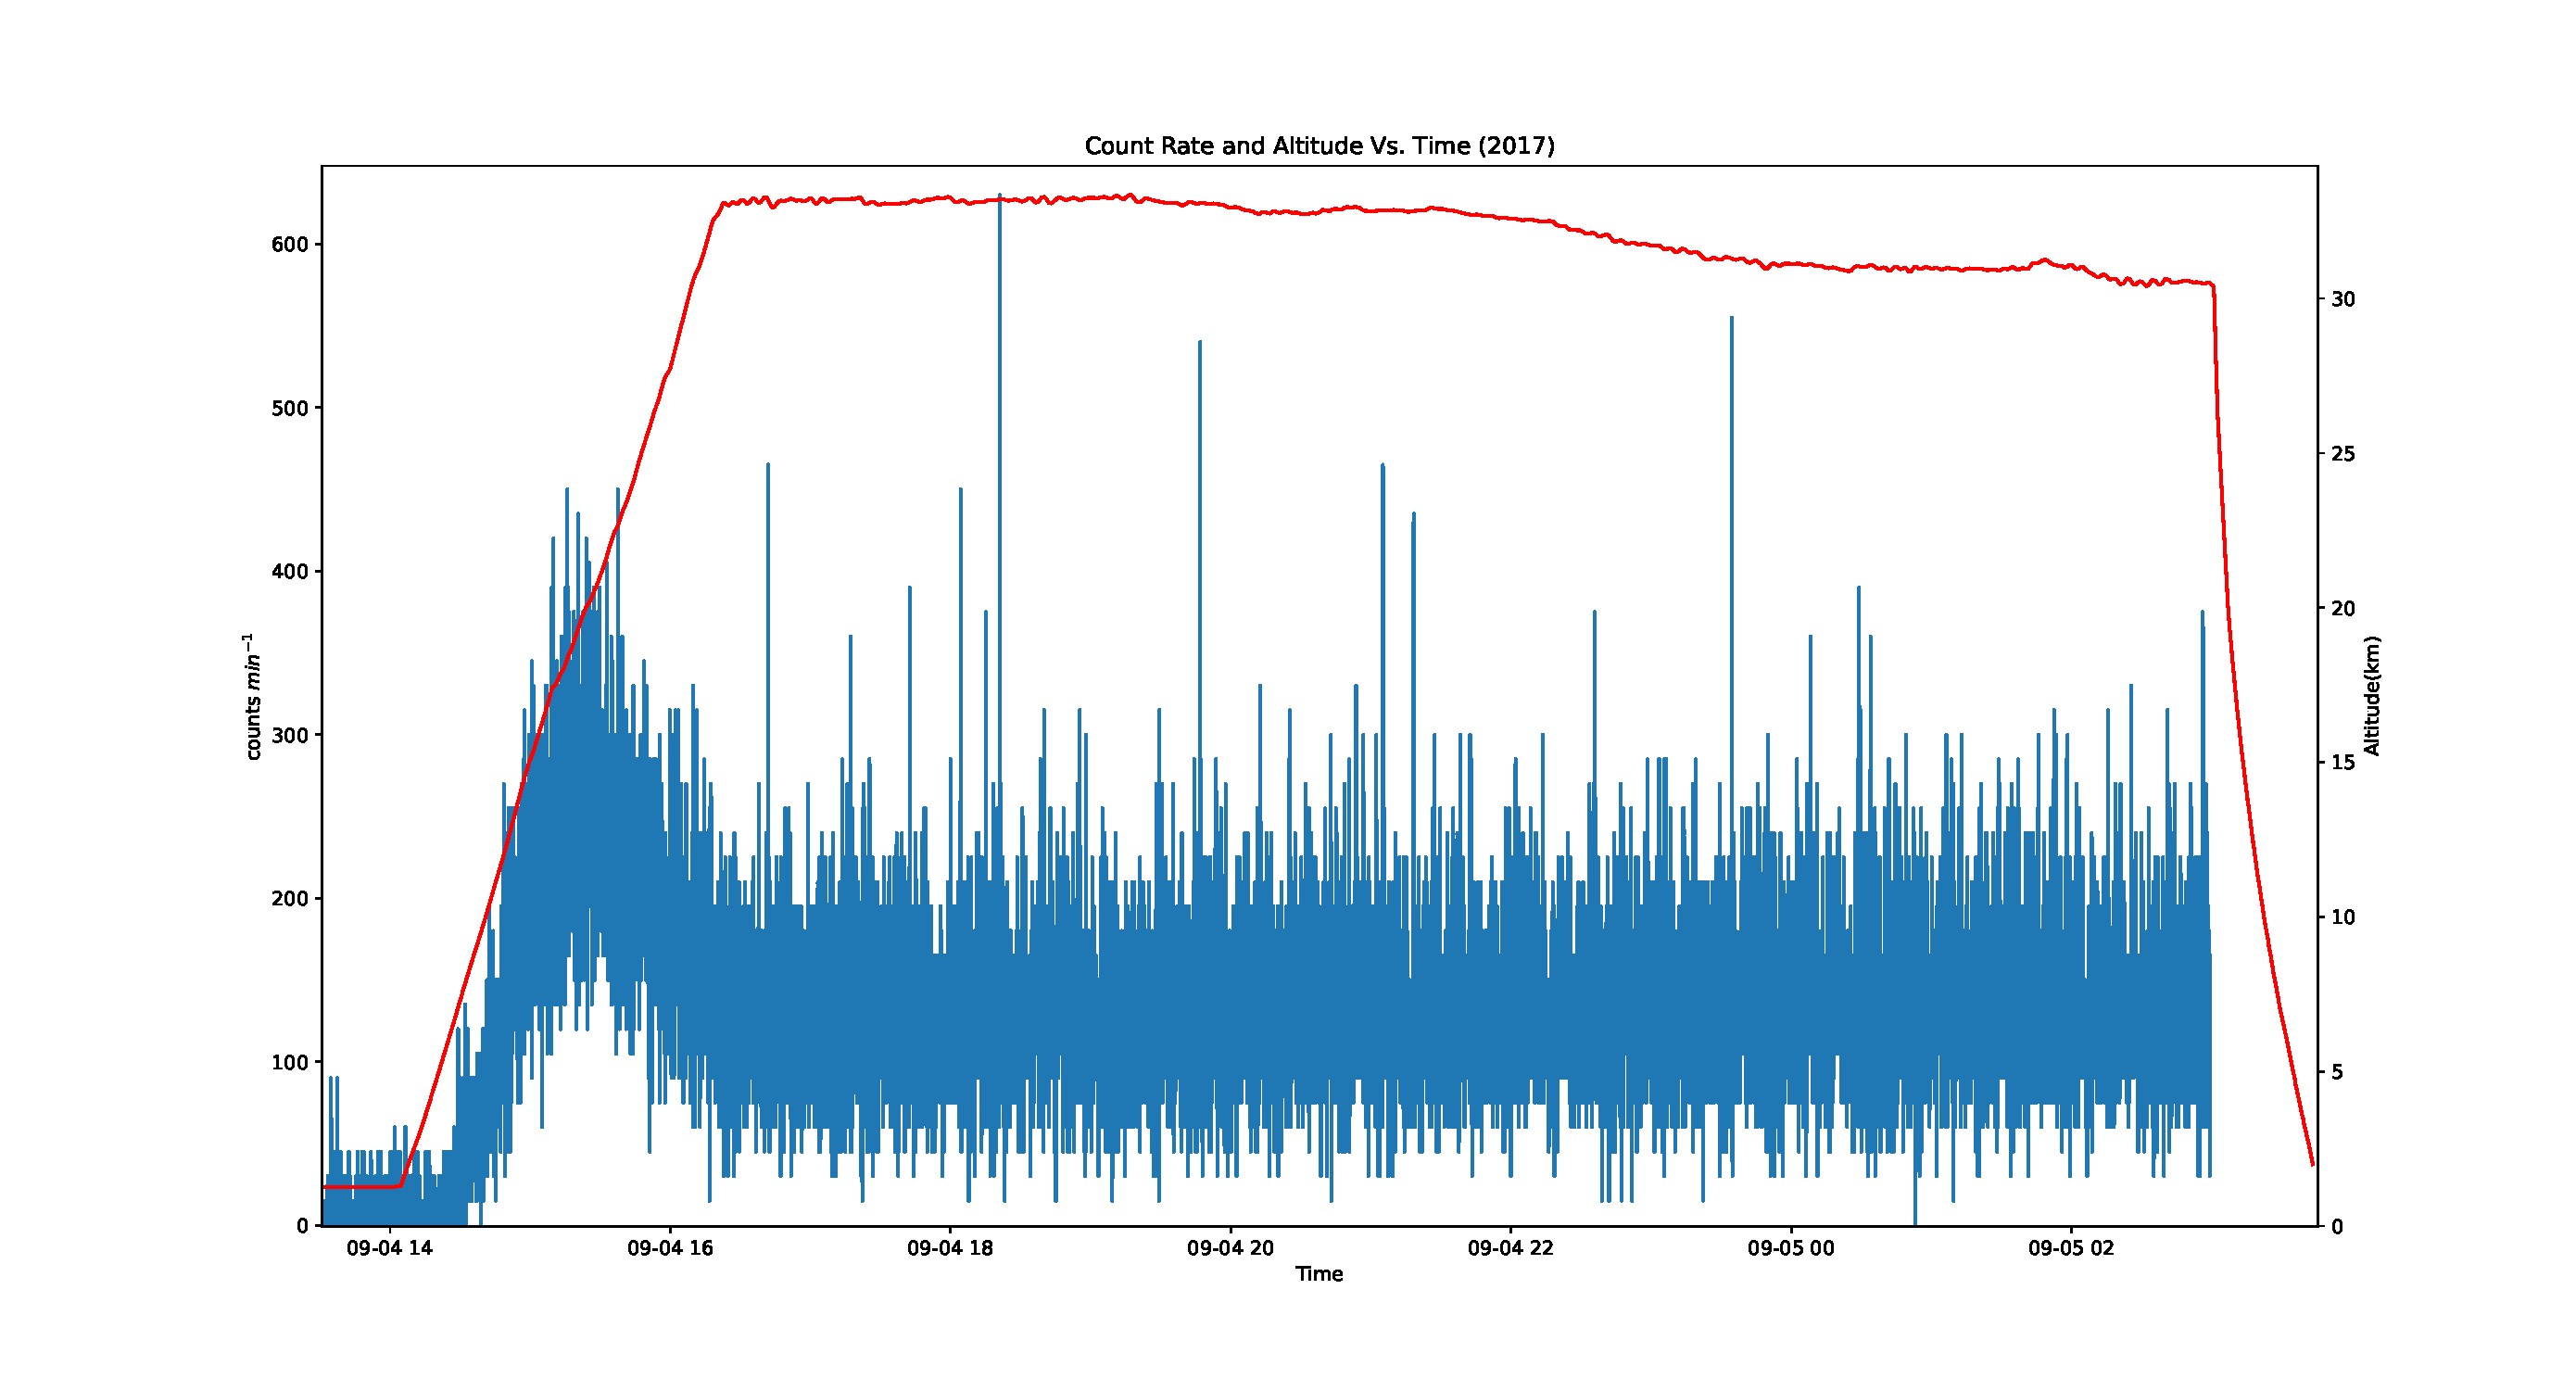
\includegraphics[scale=.45]{count_rate_altitude_2017.pdf}
\caption{Count Rate and Altitude vs Time for 2017 flight}
\label{fig:ratealttime_2017}
\end{figure}
%
%First:
%Present and characterize the first two plots - the data of the flight with counts vs altitude vs time.  Here we can talk about each flight and data shown.  Make sure to mention how the count rate changed as time and altitude changed.  We can talk about the flight time, the flight altitude variance, the coasting altitude, and how it all compares to the count rate.  We can be as descriptive as we can.
%mention the position of the pfotzer-regener maximum for both years.  Talk about discrepancies as the data shows.  Speculate in discussion later.
Both HASP balloons containing the SORA payloads were launched separately on September 4th on 2017 and 2018 respectively.  The MiniPIX was set to operate in Time over Threshold mode with a bias voltage of 4 Kev.  Frames were collected at static 4 second intervals during the 2017 flight and between 1 and 4 second intervals for the 2018 flight.  The complete flight altitude profiles and count rates for the SORA  2017 and 2018 flights are shown in Figure~\ref{fig:ratealttime_2017} and Figure~\ref{fig:ratealttime_2018} respectively.
%
\begin{figure}[H]
\centering
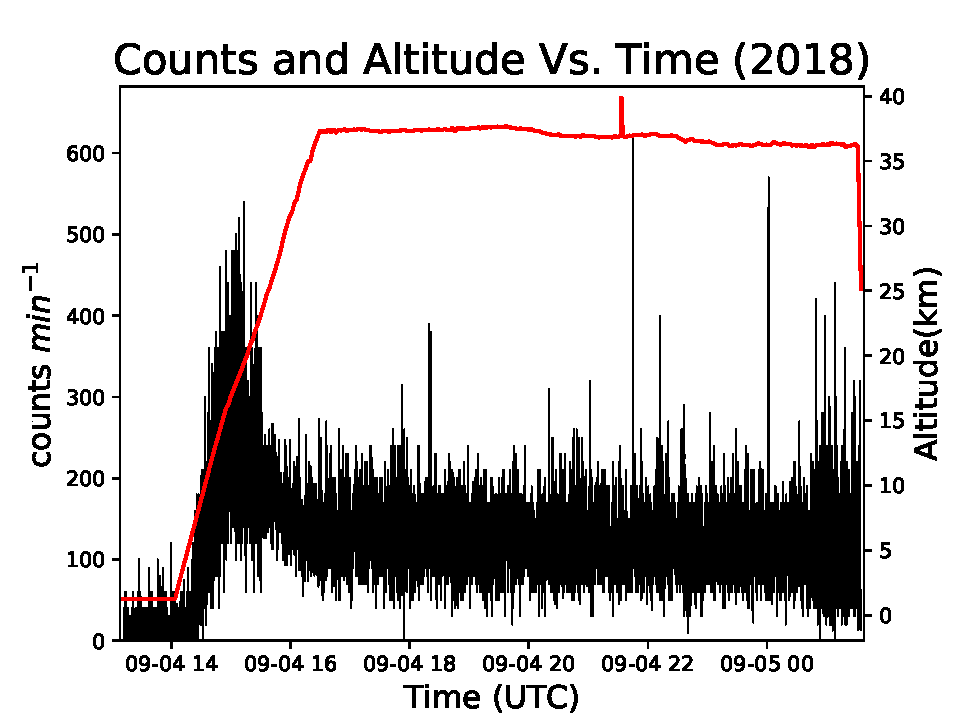
\includegraphics[scale=.50]{count_rate_altitude_2018.pdf}
\caption{Count Rate and Altitude vs Time for 2018 flight}
\label{fig:ratealttime_2018}
\end{figure}
%
As shown in Figure~\ref{fig:ratealttime_2017} and Figure~\ref{fig:ratealttime_2018}, both flights have very similar flight profiles.  Both flights reached a float altitude after approximately \SI{2.5}{\hour}.  It is important to mention that the 2017 flight reach and maintained a float altitude of approximately $\SI{31.5}{\kilo\meter}$.  In contrast, the 2018 flight kept a float altitude of $\SI{37.2}{\kilo\meter}$.  The rate of decent was slow and steady for both flights.  As such, data was collected continuously throughout the whole flights.
%

\begin{figure}[H]
\centering
\begin{subfigure}{.5\textwidth}
  \centering
  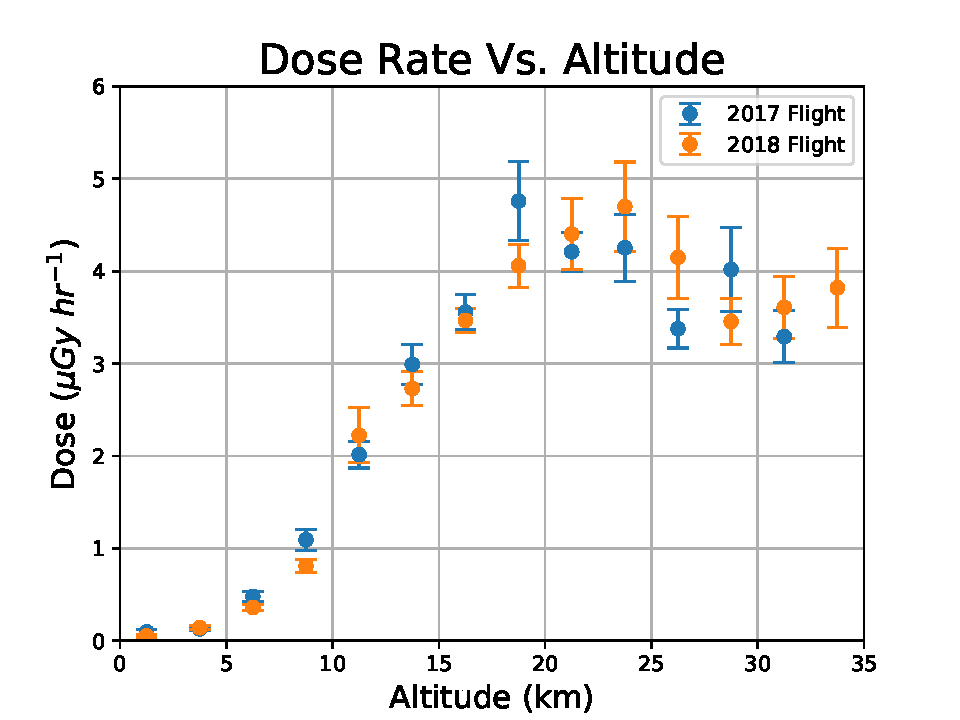
\includegraphics[scale=.45]{dva_stderr.pdf}
  \caption{Dose rate in silicon vs. altitude.}
  \label{fig:sub1}
\end{subfigure}%
\begin{subfigure}{.5\textwidth}
  \centering
  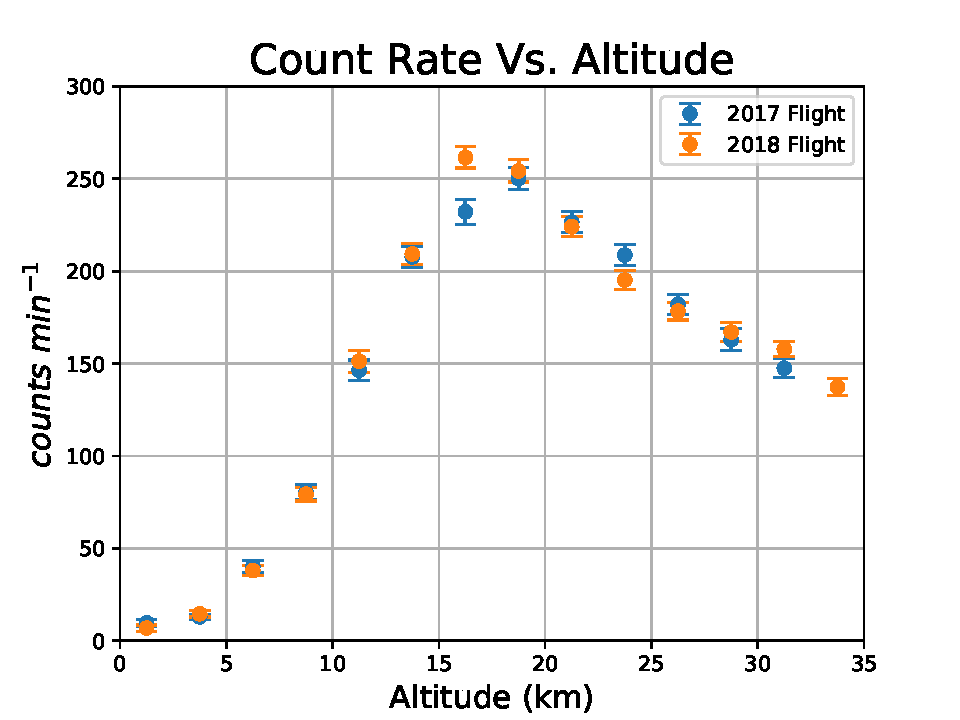
\includegraphics[scale=.45]{cva_stderr.pdf}
  \caption{Detector Hits vs. altitude.}
  \label{fig:sub2}
\end{subfigure}
\caption{Figure ~\ref{fig:sub1} shows the absorbed dose rate in silicon as a function of barometric altitude.  Figure ~\ref{fig:sub2} shows the detector counts per minute as a function of barometric altitude. Samples were averaged over \SI{2.5}{\kilo\meter} bins and error bars for both plots represent the standard error of the mean plotted at the $1\sigma$ level. }
\label{fig:sub2}
\end{figure}
%Next, go into the absorbed rate vs altitude plot.  Mention how the LET varies for materials such as silicon and muscle.  Go into the pfotzer-regener maximum again, compare.  Compare this to the accompanying figure, Detector Hits vs Altitude.  There is a slight discrepancy in the flights, this may be useful to mention.  All error bars are 1 sigma standard deviation.
Shown in Figure~\ref{fig:sub1} and Figure~\ref{fig:sub2} are dose rate in Silicon and the detector count rate plotted as a function of barometric altitude. For the sake of clarity samples were averaged over \SI{2.5}{\kilo\meter} bins and plotted with error bars representing the standard error of the mean at the $1\sigma$ level. Dose rates for both flights appear to be in relatively good agreement up until approximately \SI{16}{\kilo\meter}. After which, the 2017 flight appears to reach a peak dose rate of \SI{4.8}{\micro\gray\per\hour} at approximately \SI{18}{\kilo\meter} while the 2017 flight seems to reach a peak of \SI{4.8}{\micro\gray\per\hour} at a higher altitude of \SI{24}{\kilo\meter}. However, the large error bars indicate that it is somewhat unclear as to where the peak dose rate occurs for both flights. The count rates for both flights seem to reflect much better agreement than the dose rates and show only a small discrepency between \SI{15}{\kilo\meter} and \SI{17.5}{\kilo\meter} where the 2018 flight experienced a count rate approximately 30 counts per minute higher than that of the 2017 flight. With both flights reaching altitudes beyond $\SI{25.0}{\kilo\meter}$, the Pfotzer-Regener maximum was clearly observed.  In 2017, the Pfotzer-Regener maximum peaked at approximately  $\SI{18}{\kilo\meter}$.  Similarly, the 2018 mission recorded Pfotzer-Regener maximum peaking around $\SI{20}{\kilo\meter}$. After these peaks in count rate, the counts per minute tapered off and varied inversely with altitude.  These count rates then remained constant throughout the remainder of the flights.

%
%The Pfotzer-Regener maximum is clearly visible between \SI{15}{\kilo\meter} and \SI{20}{\kilo\meter} for both years in both absorbed dose and count rate. 
%
%Variation year over year in measurements of absorbed dose and counts is to be expected and is likely a reflection of the ongoing solar minimum. (need to expand on this a little...)
%
%Another area for the discussion - great area to talk about the discrepancies.  Here we only talk about data and thats it.
%
%Similarly, Figure~\ref{fig:sub2} again confirms the Pfotzer maximum reached for both years.
%For discussion: Here the error is more consistent and Pfotzer maximum is reached at the expected altitudes.

\begin{figure}[H]
\centering
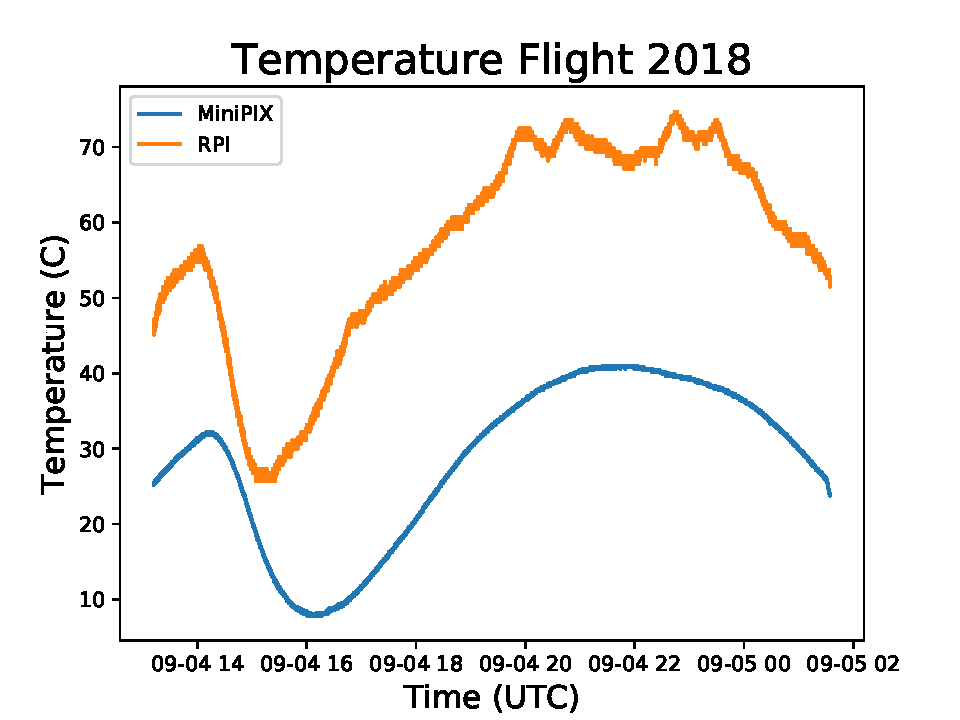
\includegraphics[width=\textwidth]{temps_flight_2018.pdf}
\caption{2018 recorded temperatures of MiniPIX and Raspberry Pi Flight computer.}
\label{fig:temps_2018}
\end{figure}
%
The MiniPIX and RPI flight computer (Raspberry Pi) both operated well throughout both flights.  The 2018 flight was better equipped to record system health and operation status.  A key status indicator of system health was the system temperature.  These temperatures recorded are shown in Figure~\ref{fig:temps_2018}.  The MiniPIX temperature stayed within expected ranges and never peaked beyond $\SI{40}{\degreeCelsius}$.  Likewise, the RPI stayed with operational temperatures.
%FOR Discussion - compare to BEXUS flights and RADX flight as well, and mention how the maximum is similar/different.  Here the maximum in the Hands et al RaD-X mission found the Pfotzer maximum around 60,000 ft (~18 km).  
%
%
%
\begin{figure}[H]
\centering
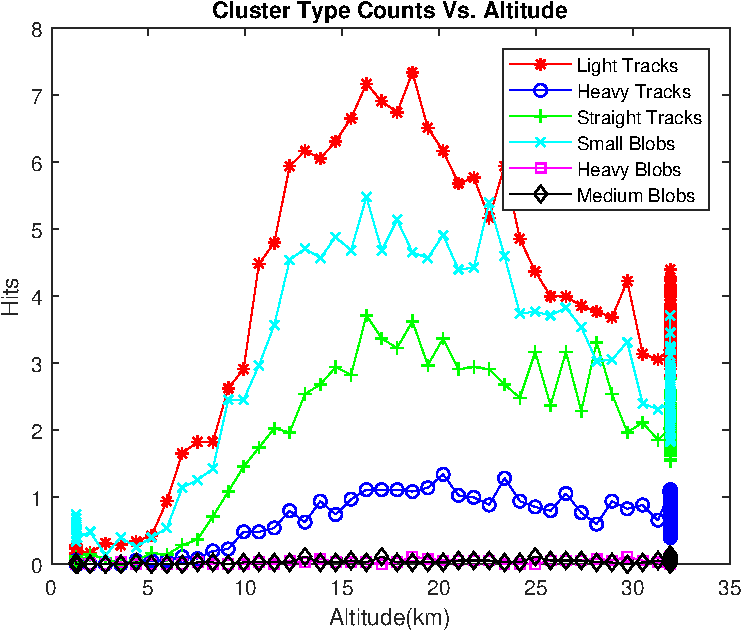
\includegraphics[width=\textwidth]{ctva-cropped.pdf}
\caption{Distribution of Cluster Type Counts vs. Altitude for the duration of the 2018 flight.}
\label{fig:cluster2018}
\end{figure}
%Finally, the last figure Cluster Type Counts vs Altitude.  This is useful due to the MiniPIX being able to analyze indivudual track lenghts.  From here, these tracks can be characterized into different and indidivual categories.  This is useful for LET calculations and overall more precise for dosage calculations.  It may also help with particle identification.
The distribution of cluster types as they vary with altitude is shown in Figure~\ref{fig:cluster2018}.  
\begin{figure}[H]
\centering
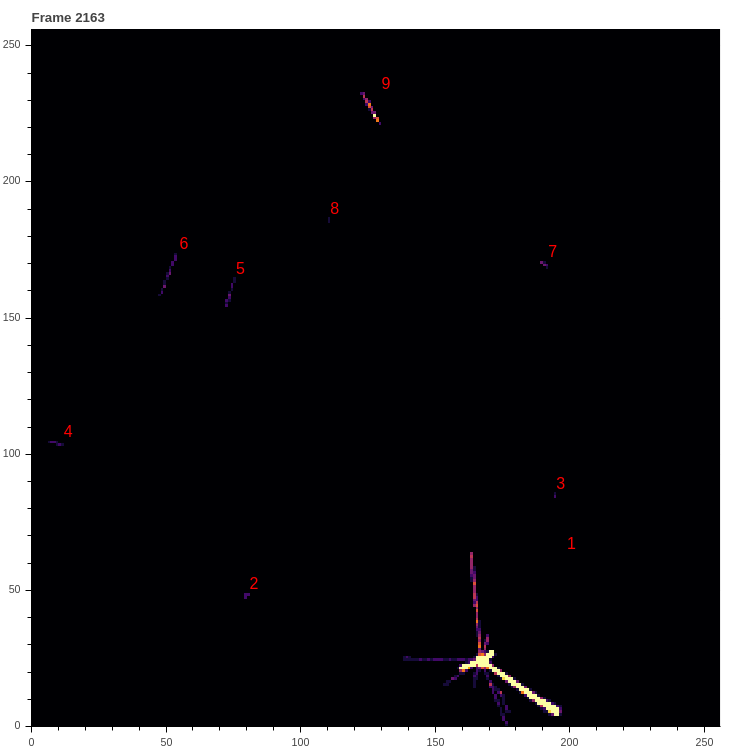
\includegraphics[width=\textwidth]{tracks.png}
\caption{Frame collected at float.}
\label{fig:frame1}
\end{figure}
Figure~\ref{fig:frame1} shows one of many particle tracks recorded during the duration of both 2017 and 2018 flights.  The track lengths of ionizing particles can be calculated and used to directly measure the linear energy transfer of various primary and secondary particles.


